\documentclass[preprint,12pt]{elsarticle}

\usepackage{amsmath,amssymb}
\usepackage{array}
\usepackage{booktabs}
\usepackage{graphicx}
\usepackage{lmodern}
\usepackage{microtype}
\usepackage{multirow}
\usepackage[hidelinks]{hyperref}
\usepackage{url}

\setlength{\emergencystretch}{2em}
\newcolumntype{L}[1]{>{\raggedright\arraybackslash}p{#1}}
\journal{Information Processing in Agriculture}

% Use a dagger for shared first authorship while retaining Elsevier's asterisk
% convention for the corresponding author.
\makeatletter
\newcommand{\equalcontribref}{\gdef\@fnmark{\ensuremath{\dagger}}}
\newcommand{\equalcontribtext}[1]{%
  \g@addto@macro\@fnotes{%
    \begingroup
    \def\thefootnote{\ensuremath{\dagger}}%
    \footnotetext{#1}%
    \endgroup}}
\makeatother
\pdfstringdefDisableCommands{\def\equalcontribref{}}

\begin{document}
\begin{frontmatter}

\title{Auditing crop host supervision in Swin models for condition recognition across multiple crops: evidence from 90 controlled runs}

\author[inst1]{Muhammad Omair Khan\equalcontribref}
\ead{mumairkhan690@gmail.com}
\author[inst1]{Muhammad Ahmad\equalcontribref}
\ead{filliones@gmail.com}
\author[inst1]{MD Ariful Islam Mozumder}
\ead{arifulislamro@gmail.com}
\author[inst2]{Hee-Cheol Kim\corref{cor1}}
\ead{heeki@inje.ac.kr}
\equalcontribtext{Muhammad Omair Khan and Muhammad Ahmad contributed equally
to this work and share first authorship.}
\cortext[cor1]{Corresponding author. Email: heeki@inje.ac.kr.}
\address[inst1]{Institute of Digital Anti-Aging Healthcare, Inje University,
Gimhae 50834, Republic of Korea.}
\address[inst2]{Department of Computer Science and Engineering, Inje University,
Gimhae 50834, Republic of Korea.}

\begin{abstract}
Classifiers covering multiple crops can return a condition that conflicts with
their own crop prediction. A separate host head reveals these conflicts,
although the host is already determined by the joint label. We tested whether host
supervision improves recognition or mainly supports model audit. A Swin Small
model pretrained on ImageNet was evaluated on three fixed benchmarks containing
43, 88, and 215 classes. Related augmentation families were confined to one
split, exact duplicates and label conflicts were checked, and flat and dual
models were paired by seed. Ten pairs were run per dataset, while two agreement
losses were evaluated with five matched seeds, giving 90 runs. Flat and dual
accuracies were 99.409 versus 99.398 percent, 97.657 versus 97.708 percent, and
92.151 versus 92.271 percent. At a predeclared margin of $\pm0.25$ percentage
points, all outcomes on the benchmark with 43 classes were equivalent. Accuracy
and cross-host error were also equivalent on the 88-class benchmark; macro F1
was unresolved. Neither agreement loss improved performance consistently across
datasets and metrics. On the benchmark with 215 classes, a labeled-host oracle increased
accuracy by about 2.2 points. Predicted-host masking removed all head conflicts
but changed mean accuracy by at most 0.018 points. Temperature scaling fitted on
validation data reduced expected calibration error from about 5.4 percent to
between 1.6 and 1.7 percent. Host supervision did not yield a dependable
accuracy gain; its clearest value was exposing internal disagreement for audit.
\end{abstract}

\begin{keyword}
Plant disease recognition \sep hierarchical classification \sep Swin Transformer
\sep model audit \sep split integrity \sep probability calibration
\end{keyword}

\end{frontmatter}

\section{Introduction}
\label{sec:introduction}

Image recognition is now used to organize crop image collections, flag likely
disease cases, and support specialist review \cite{mohanty2016,gui2021}. A
system that covers several crops must do more than choose a condition label. Its
crop and condition outputs should agree, and the reported confidence should be
useful when a prediction is accepted or sent for review. For example, a model
may assign a tomato condition while its crop head selects grape. The condition
may still be correct, but the model has produced two incompatible descriptions
of the same image.

Many plant image datasets encode crop and condition in one joint class, such as
\texttt{Tomato\_\_late\_blight}. A flat classifier treats these classes as an
ordinary list. A second head can predict the crop host from the shared image
features and can identify conflicts across the taxonomy. The extra target,
however, is not independent in the datasets examined here. Once the joint class
is known, the crop host follows from a fixed mapping. The host task repeats part
of the original label, so an improvement cannot be assumed. A related concern
applies to masking. Restricting condition classes to the crop predicted by the
host head always produces a compatible pair, but an incorrect host prediction
can remove the correct condition from consideration.

Small changes in benchmark accuracy are also easy to misread. Augmented copies
of one photograph can enter different splits, exact duplicates can carry
conflicting labels, and a favorable random seed can make one model appear
better than another. Model rankings may change with initialization, data order,
and other sources of training variation \cite{bouthillier2021}. A sound
comparison needs fixed split identities, paired runs, uncertainty for the
paired difference, and a stated threshold for an effect that is too small to
matter in practice. A nonsignificant test alone does not establish that two
models perform similarly.

We asked whether deterministic crop host supervision adds useful evidence to a
Swin model that predicts joint crop conditions. We addressed five questions.
First, we compared condition accuracy, macro F1, and cross-host error between
flat and dual models. Second, we tested practical equivalence at a margin
declared before analysis and checked two alternative margins. Third, we
evaluated MAE and $\mathrm{KL}(q\|p^h)$ agreement losses. Fourth, we measured
disagreement between the two heads before and after predicted-host masking, and
compared the masking result with a labeled-host oracle that is unavailable at
deployment. Finally, we examined calibration and selective error using
temperatures fitted only on validation data.

The contribution lies in the controlled evaluation rather than in a new image
backbone. Each flat and dual comparison used the same Swin Small representation,
optimizer, split, and seeds. The three taxonomies differ markedly in size and
imbalance, which lets us examine when the host head becomes more active and
whether that activity improves the primary prediction. All conclusions refer
to the fixed datasets used here. They do not establish performance on new
farms, cameras, seasons, or geographic regions.

\section{Related work}
\label{sec:related}

\subsection{Recognition of crop conditions from images}

PlantVillage made controlled evaluation of plant disease classifiers easier to
reproduce \cite{hughes2015,mohanty2016}. Convolutional networks later reached
high accuracy on curated leaf images \cite{ferentinos2018}, while subsequent
work showed that dataset size, background, visual diversity, and acquisition
conditions strongly affect transfer beyond the source collection
\cite{barbedo2018,gui2021}. Vision Transformers and shifted-window
Transformers provide strong pretrained representations for image recognition
\cite{dosovitskiy2021,liu2021swin}. An improved Vision Transformer has also
been tested for crop pest recognition in this journal \cite{fu2024}. We chose
Swin Small as a common pretrained backbone so that the comparison focuses on
the host target and not on a new feature extractor.

\subsection{Hierarchical labels and auxiliary tasks}

Multitask learning can help when an auxiliary target contributes information
that supports the main task \cite{caruana1997}. Hierarchical classification
uses known relations among labels to organize predictions or prevent invalid
outputs \cite{silla2011}. Previous studies have used crop identity as metadata,
an intermediate prediction, or an additional target in conditioned networks
and models with multiple outputs \cite{picon2019,yao2024}. Our setting is
narrower. Every host target can be recovered exactly from the joint condition
label. The experiment therefore asks whether repeating that information changes
the learned decision under otherwise matched training. It also separates an
accurate prediction from one made valid by a rule after the model has produced
conflicting outputs.

\subsection{Evidence needed for a model audit}

Agricultural image studies increasingly report more than overall accuracy.
Recent reviews in this journal note that data composition and evaluation choices
shape the conclusions drawn from plant health models \cite{ngugi2021,elhanafy2026}.
Erg\"un and Okumu\c{s} studied an adaptive ensemble on imbalanced eggplant data
\cite{ergun2026}. Singh et al. combined deduplication, calibration, and
agronomic rule checks for rice disease diagnosis \cite{singh2026}. Outside
agriculture, identity leakage has been linked to optimistic estimates in
machine learning research \cite{kapoor2023}.

This leaves a practical question. When part of a hierarchy is deterministic,
does the auxiliary level improve the primary decision, or does it simply
provide another view of the same output? We combine source identity controls,
paired replication, equivalence tests, head disagreement rate (HDR), taxonomic
consistency inference (TCI), a labeled-host oracle, and calibration.
Table~\ref{tab:related-audit-comparison} places these elements beside selected
studies that condition on crop identity, use several outputs, or apply rule
checks.

\begin{table*}[htbp]
\centering
\caption{Positioning against representative crop-condition studies. ``NR''
means that the cited article did not report the item as an explicit analysis;
it does not establish that the underlying data or code lacked the property.}
\label{tab:related-audit-comparison}
\scriptsize
\setlength{\tabcolsep}{2.5pt}
\begin{tabular}{@{}L{0.11\textwidth}L{0.13\textwidth}L{0.17\textwidth}
                    L{0.13\textwidth}L{0.07\textwidth}L{0.16\textwidth}
                    L{0.11\textwidth}@{}}
\toprule
Study & Data setting & Hierarchy design & Identity control & Paired seeds & Equivalence / calibration & Constraint audit\\
\midrule
Mohanty et al.\ \cite{mohanty2016} & Controlled PlantVillage images & Joint crop and condition CNN & NR & NR & NR / NR & NR\\
Picon et al.\ \cite{picon2019} & Multi-crop field images & Crop-metadata-conditioned CNN & NR & NR & NR / NR & NR\\
Yao et al.\ \cite{yao2024} & Three benchmark datasets & Multi-output and stacked CNNs & NR & NR & NR / NR & NR\\
Fu et al.\ \cite{fu2024} & Crop-pest image benchmark & Improved ViT classifier & NR & NR & NR / NR & NR\\
Erg\"un and Okumu\c{s} \cite{ergun2026} & Three eggplant benchmarks & Learned CNN ensemble and TTA & NR & NR; CV & No / NR & NR\\
Singh et al.\ \cite{singh2026} & PaddyDoctor rice images & Post-hoc agronomic rule validator & Perceptual-hash deduplication & NR & No / temperature scaling & Rule contradictions\\
This study & Three fixed in-domain benchmarks & Auxiliary host head and masking & Original-family and/or exact-hash controls & 10 paired & TOST, Holm, margin sensitivity / scaling & HDR, TCI, oracle host\\
\bottomrule
\end{tabular}
\end{table*}


\section{Materials and methods}
\label{sec:methods}

\subsection{Study design}
\label{sec:design}

The three datasets were analyzed separately. No image moved from one benchmark
to another. Split manifests and ordered mappings from conditions to hosts were
fixed before model training. Each primary comparison paired a flat model and a
dual model with the same seed. The two agreement losses were secondary analyses
with fixed coefficients; their settings were not selected from test results.
Figure~\ref{fig:workflow} shows the data flow, Swin Small backbone, prediction
heads, training losses, and locked test analyses.

\begin{figure*}[htbp]
\centering
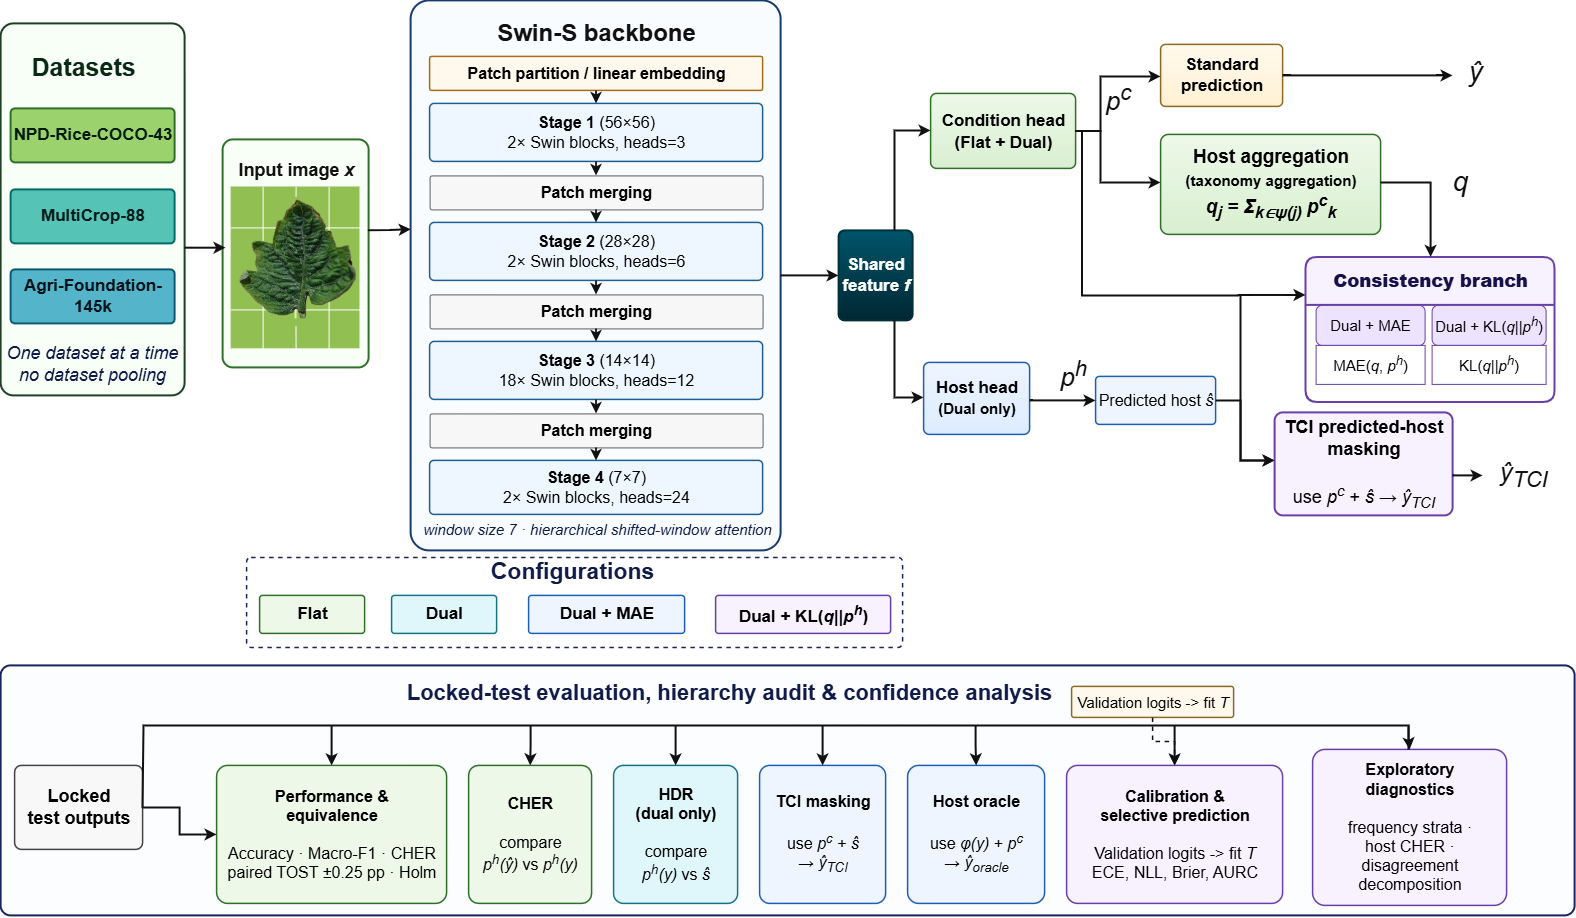
\includegraphics[width=\textwidth]{fig01_workflow_architecture.png}
\caption{Study workflow and model architecture. A $224\times224$ image passes
through the four stages of Swin Small, with stage depths 2, 2, 18, and 2 and
attention head counts 3, 6, 12, and 24. Every configuration has a condition
head. Dual configurations also have a host head. Condition probabilities are
summed within the fixed taxonomy to form the condition-implied host
distribution $q$. The MAE and $\mathrm{KL}(q\|p^h)$ branches add differentiable
agreement losses during training. TCI restricts the condition decision to the
host selected by the direct host head. Locked test outputs are used for
performance, equivalence, CHER, HDR, TCI, the labeled-host oracle, calibration,
selective risk, and analyses by class frequency. CHER is the cross-host error
rate; HDR is the head disagreement rate; TOST refers to two one-sided tests; ECE
is expected calibration error; NLL is negative log likelihood; and AURC is the
area under the risk-coverage curve. The workflow schematic was prepared with
assistance from an LLM and was subsequently checked and edited by the authors.}
\label{fig:workflow}
\end{figure*}

\subsection{Datasets and split integrity}
\label{sec:data}

Each image had one joint crop and condition label $y$. A fixed mapping
$\phi(y)$ assigned that class to a host group. We use \emph{condition} rather
than \emph{disease} because the label sets also include healthy states, pests,
nutrient disorders, and one supervised non-plant category.

\paragraph{NPD-Rice-COCO-43}
The first benchmark was assembled locally from three public sources. The New
Plant Diseases Dataset was the main component and contributed 87,425 local
image paths in 38 crop-condition classes \cite{newplantdiseases}. The Rice
Leafs Dataset contributed all 3,355 local images in four classes: Brown Spot,
Healthy, Hispa, and Leaf Blast \cite{riceleafs}.

To provide a supervised non-plant background category, a subset of 2,608 images
was additionally selected from the COCO 2014 dataset
\cite{lin2014,coco2014kaggle}. COCO was not used as an agricultural data source
and did not contribute any plant-disease classes. Instead, the selected images
represented unrelated visual content, including people, animals, and common
everyday objects, and were grouped into a single non-plant background class.
The purpose of this auxiliary category was to reduce the tendency of the
classifier to assign clearly non-plant inputs to one of the crop-condition
classes. Because these images were included during model training, this
category is treated as a supervised background class rather than as an open-set
or out-of-distribution evaluation. In the resulting NPD-Rice-COCO-43 benchmark,
the COCO-derived category therefore constitutes one auxiliary non-plant class
alongside the 42 crop-condition classes obtained from the New Plant Diseases
Dataset and the Rice Leafs Dataset.

The complete benchmark contained 93,388 image paths, 43 prediction classes,
and 16 taxonomy groups. The supplied archive does not retain the original COCO
sampling script. We therefore make no unverified claim about category balance
or a formal adversarial sampling rule for the selected background images.

The packaged source directories were pooled and split deterministically in an
80, 10, and 10 percent ratio. Augmented files linked by a source UUID or a
normalized stem before augmentation were assigned together. Rice files with
the same source stem and COCO files with the same image identifier were also
kept together. Exact byte duplicates were joined to the same assignment group.
No exact hash appeared with conflicting labels, and no path was removed.

\paragraph{MultiCrop-88}
This local composite was derived from the Kaggle Plant Disease Classification
Merged Dataset \cite{dobrovsky_multicrop}. It initially contained 79,086 image
paths in 88 classes and 23 host groups. The benchmark is also consistent with
the multi-crop disease setting considered by Ahamed et al. \cite{ahamed2024}.
We removed 1,254 redundant same-label paths from 1,232 exact-hash clusters. A
further 62 paths from 29 hashes were excluded because the same bytes carried
different labels. The 77,770 remaining images were divided deterministically
into 80, 10, and 10 percent partitions with every class present in each
partition. Because the Kaggle package does not provide original acquisition or
augmentation-family identifiers, \texttt{family\_id} records an exact-hash
assignment unit rather than an independently verified biological or acquisition
family.

\paragraph{Agri-Foundation-145k}
The Hugging Face distribution used locally and the permanent Zenodo record
describe Agri-Foundation-145k as a 215-class agricultural disease dataset
\cite{agrifoundation_hf,agrifoundation2026}. The locked local derivative
contained 144,752 paths
in 215 classes and 36 host groups. It had 92,571 training images, 23,140
validation images, and a separate test set of 29,041 images. The one-path
difference came from a synthetic $10\times10$ file named \texttt{dummy.jpg}.
This file was the only development example for one joint class and is not an
observed plant image. It was retained because the reported runs had already
been completed with that locked derivative. The exact-hash audit found no match
between the development pool and the test set. All 215 classes occurred in
training and test, while 212 occurred in validation. Results for the class that
contains the placeholder, and its contribution to absolute macro F1, require
special caution. Since every configuration used the same derivative, the
paired comparison remains case matched.

Table~\ref{tab:split-audit} reports the final counts and the identity checks.
For NPD-Rice-COCO-43, no assignment group, source family, or SHA-256 hash crossed
a split. For MultiCrop-88, no assignment group or exact hash crossed a split.
Exact hashes do not identify near duplicates created by resizing, compression,
cropping, or other image transformations. No perceptual hash or embedding
similarity audit was available for MultiCrop-88 or Agri-Foundation-145k.

\begin{table*}[htbp]
\centering
\caption{Dataset counts and split integrity checks. Counts refer to paths after
the stated exclusions. The local Agri-Foundation-145k total is one path above
the public record because of the disclosed development placeholder.}
\label{tab:split-audit}
\small
\resizebox{\textwidth}{!}{%
\begin{tabular}{lrrrrrrl}
\toprule
Dataset & Hosts & Classes & Train & Validation & Test & Excluded & Integrity control\\
\midrule
NPD-Rice-COCO-43 & 16 & 43 & 74,700 & 9,355 & 9,333 & 0 &
Source-family grouping; zero overlap by family or hash\\
MultiCrop-88 & 23 & 88 & 62,214 & 7,787 & 7,769 & 1,316 &
Exact deduplication; conflicting hashes excluded\\
Agri-Foundation-145k & 36 & 215 & 92,571 & 23,140 & 29,041 & 0 &
Fixed split; one development placeholder; zero exact development-to-test overlap\\
\bottomrule
\end{tabular}%
}
\end{table*}

\subsection{Flat and host-aware Swin models}
\label{sec:model}

The backbone used the exact \texttt{timm} weight identifier
\path{swin_small_patch4_window7_224.ms_in22k_ft_in1k}. These weights were
obtained by pretraining on ImageNet 22k followed by fine-tuning on ImageNet 1k
\cite{russakovsky2015}. Swin Small divides a $224\times224$ image into
$4\times4$ patches, then applies four shifted-window stages with depths
$(2,2,18,2)$ and attention head counts $(3,6,12,24)$. The final representation
$\mathbf f$ has 768 dimensions \cite{liu2021swin}. The flat model has one
linear condition head. The dual model adds a separate host head:
\begin{equation}
 \mathbf z^c=W_c\mathbf f+b_c,\qquad
 \mathbf z^h=W_h\mathbf f+b_h.
\end{equation}
The added head contains $(768+1)S$ trainable parameters. This corresponds to
12,304 parameters for 16 hosts, 17,687 for 23 hosts, and 27,684 for 36 hosts.
The backbone is identical in the two models.

Softmax gives condition probabilities $\mathbf p^c$ and direct host
probabilities $\mathbf p^h$. Condition probabilities are also summed within the
taxonomy to obtain a host distribution implied by the condition head:
\begin{equation}
 q_j=\sum_{k:\phi(k)=j}p^c_k,\qquad j=1,\ldots,S.
 \label{eq:aggregation}
\end{equation}
Standard inference selects $\hat y=\arg\max_k p^c_k$ and independently selects
$\hat s=\arg\max_j p^h_j$. TCI was examined as a secondary analysis. It masks
all condition classes outside the directly predicted host:
\begin{equation}
 \hat y_{\mathrm{TCI}}=\arg\max_{k:\phi(k)=\hat s}p^c_k.
 \label{eq:tci}
\end{equation}
This rule needs no retraining and always returns a condition that belongs to the
reported host. It cannot guarantee that either prediction is correct.

The flat loss was condition cross entropy. The dual loss added host cross
entropy with a fixed weight of one:
\begin{equation}
 \mathcal L_{\mathrm{dual}}=
 \operatorname{CE}(\mathbf z^c,y)+
 \alpha\operatorname{CE}(\mathbf z^h,\phi(y)),\qquad \alpha=1.
 \label{eq:dual}
\end{equation}
Two additional variants encouraged agreement between $\mathbf q$ and
$\mathbf p^h$:
\begin{align}
 \mathcal L_{\mathrm{MAE}}&=\frac{1}{S}\sum_{j=1}^{S}|q_j-p^h_j|,\\
 \mathcal L_{\mathrm{KL}(q\|p^h)}&=\sum_{j=1}^{S}q_j
 \left[\log\{\max(q_j,\epsilon)\}-
 \log\{\max(p^h_j,\epsilon)\}\right].
\end{align}
The full loss was $\mathcal L_{\mathrm{dual}}+\lambda
\mathcal L_{\mathrm{MAE}}$ or $\mathcal L_{\mathrm{dual}}+\lambda
\mathcal L_{\mathrm{KL}(q\|p^h)}$, with $\lambda=1$. MAE was averaged over
samples and host categories. KL was summed over host categories and averaged
over samples. The numerical floor was
$\epsilon=\texttt{torch.finfo}(\mathbf p^h.\texttt{dtype}).\texttt{eps}$.
The condition-implied distribution was not detached, so both heads received
gradients from the agreement term. The unit coefficients were fixed and do not
equalize the gradient scales of MAE and KL.

\subsection{Training protocol and experiment matrix}
\label{sec:training}

Every run started from the same pretrained Swin Small weights. We used AdamW
\cite{loshchilov2019}, a learning rate of $10^{-4}$, weight decay of
$10^{-4}$, batch size 16, cosine annealing without warmup, and 30 epochs. The
training transform used a random resized crop to $224\times224$ pixels with a
scale from 0.5 to 1.0, a random horizontal flip, and color jitter of 0.2 for
brightness, contrast, and saturation. Validation and test images were resized
to 256 pixels, center-cropped to $224\times224$, and normalized with ImageNet
statistics. The checkpoint with the highest validation macro F1 was retained.

Training used CUDA automatic mixed precision. Selected checkpoint weights were
stored in FP32. The primary runs exported FP32 validation and test logits for
calibration. Saved predictions were used for the discrete hierarchy analyses,
and logits were used when available. Seeds controlled initialization, data
order, and augmentation. Deterministic PyTorch and cuDNN behavior was enabled,
\texttt{CUBLAS\_WORKSPACE\_CONFIG=:4096:8} was set, and random number states
were stored for resumed runs.

Flat and dual models used seeds 2026 to 2035 on each dataset. The MAE and KL
variants used seeds 2026 to 2030 and were compared with dual controls using the
same five seeds. This produced 30 runs for each dataset and 90 runs in total
(Table~\ref{tab:matrix}). Every retained run completed all 30 epochs.

\begin{table}[htbp]
\centering
\caption{Experiment matrix. Each seed represents a separate fine-tuning run.}
\label{tab:matrix}
\small
\resizebox{\columnwidth}{!}{%
\begin{tabular}{lccc}
\toprule
Configuration & Objective & Seeds per dataset & Runs\\
\midrule
Flat & Condition CE & 10 & 30\\
Dual & Condition CE plus host CE & 10 & 30\\
Dual plus MAE & Dual loss plus MAE agreement & 5 & 15\\
Dual plus $\mathrm{KL}(q\|p^h)$ & Dual loss plus KL agreement & 5 & 15\\
\midrule
Total & & & 90\\
\bottomrule
\end{tabular}%
}
\end{table}

\subsection{Outcomes and hierarchy diagnostics}
\label{sec:outcomes}

The primary outcomes were top-1 condition accuracy, macro F1, and cross-host
error rate (CHER). Macro F1 was the unweighted mean over all condition classes;
a class received zero when its F1 value was undefined. CHER counts a condition
prediction as a cross-host error when it belongs to a different host from the
label:
\begin{equation}
 \mathrm{CHER}=\frac{1}{N}\sum_{i=1}^{N}
 \mathbb 1[\phi(\hat y_i)\ne\phi(y_i)].
 \label{eq:cher}
\end{equation}
For dual models, HDR compares the host implied by the condition argmax with the
host selected by the direct host head:
\begin{equation}
 \mathrm{HDR}=\frac{1}{N}\sum_{i=1}^{N}
 \mathbb 1[\phi(\hat y_i)\ne\hat s_i].
 \label{eq:hdr}
\end{equation}
HDR measures internal agreement. CHER compares the condition prediction with
the labeled host. Host accuracy and HDR were calculated for all 60 dual runs.
TCI was then applied to the same locked outputs, and we recorded its change in
accuracy, macro F1, and CHER. HDR and TCI are not defined for the flat model.
Unless noted otherwise, metrics are reported as percentages.

We ran additional descriptive analyses on the benchmark with 215 classes.
Classes were grouped by training support: 1 to 25, 26 to 100, 101 to 500, and
more than 500 images. Class F1 was averaged within each group for every seed.
CHER was also summarized by labeled host. A labeled-host oracle masked fixed
condition logits to classes compatible with the true host before taking the
argmax. The oracle sets CHER to zero and is not deployable; it estimates how
much error lies across host boundaries. For the dual model without an agreement
loss, each head disagreement was classified according to whether the direct
host, the condition-implied host, or neither matched the label. We also counted
correct predictions gained and lost after TCI. These analyses were exploratory
and were not included in the adjusted superiority tests.

\subsection{Calibration and statistical analysis}
\label{sec:statistics}

Within each dataset, flat and dual outcomes were paired by seed. We calculated
the mean dual minus flat difference and a 95 percent confidence interval based
on the paired $t$ distribution. Before examining the differences, we defined
practical equivalence as an effect inside $\pm0.25$ percentage points. For
accuracy, this is one changed decision in 400 images. We applied the same
absolute margin to macro F1 and CHER so that the threshold was not widened after
seeing the results.

Equivalence was tested with two one-sided tests using a 90 percent interval.
The nine decisions formed by three datasets and three metrics were adjusted by
the Holm procedure \cite{lakens2017,holm1979}. We declared equivalence only
when the entire 90 percent interval lay within the margin and the adjusted test
passed at $\alpha=0.05$. An outcome that did not pass was called unresolved;
it was not treated as evidence that the models differ. The same nine-decision
adjustment was repeated after analysis at margins of $\pm0.10$ and $\pm0.50$
points. We also translated each CHER margin into a number of errors on the fixed
test set. These intervals describe variation across fine-tuning seeds for one
test set. They do not represent repeated sampling from a new population.

NPD-Rice-COCO-43 contains different numbers of augmented files per source
family. As a sensitivity check, every test family received total weight one.
Each image was weighted by the inverse of its family size, and weighted
accuracy, macro F1, and CHER were calculated for each seed before the paired
summary. This changed the contribution of repeated augmentations without
changing the models or test cases.

The five-seed comparisons of agreement losses were secondary. We report paired
95 percent intervals but do not use them for a general claim of superiority.

Probability quality was evaluated for all 60 primary flat and dual checkpoints.
A single temperature was fitted to validation logits by minimizing negative log
likelihood (NLL) and then applied once to the locked test logits
\cite{guo2017}. We report expected calibration error (ECE) from 15 top-label
bins, NLL, the summed multiclass Brier score \cite{brier1950}, and area under
the risk-coverage curve (AURC) \cite{geifman2017}. Lower values are better.
Risk-coverage curves rank images by maximum calibrated condition probability
and calculate the error among the retained highest-confidence fraction.
Temperature scaling changes probability magnitude but normally leaves the
predicted class and its ordering by confidence unchanged.

\subsection{LLM support in the research workflow}
\label{sec:ai-methods}

An assistant based on a large language model (LLM) supported code review,
internal consistency checks, manuscript organization, language editing, and
preparation of the workflow schematic. The LLM did not generate training
images, experimental measurements, model predictions, or statistical decisions.
The authors inspected the implementation, checked the references, and matched
every reported value to the stored outputs. They take responsibility for the
final methodology, analysis, and presentation.

\section{Results}
\label{sec:results}

\subsection{Integrity checks and completed runs}

The reconstructed NPD-Rice-COCO-43 and MultiCrop-88 partitions passed all
specified exact identity checks. NPD-Rice-COCO-43 had no overlap across
partitions by assignment group, source family, or SHA-256 hash. MultiCrop-88
retained 77,770 unique images after 1,316 exclusions and had no shared
assignment group or hash across partitions. Its hash-derived
\texttt{family\_id} should not be interpreted as independent source provenance.
The Agri-Foundation-145k test set had no exact hash match with the development
pool. The development placeholder described in Section~\ref{sec:data} remained
in the locked local derivative.

All 90 runs completed 30 epochs and passed the available checks of
configuration, identity, and output files. Each run recorded the intended
dataset, seed, model configuration, checkpoint history, and locked test
predictions. FP32 validation and test logits were available for every primary
flat and dual run.

\subsection{Flat and dual performance}
\label{sec:core-results}

Table~\ref{tab:critical-core-results} gives the main test results.
NPD-Rice-COCO-43 was close to saturation. The dual model changed accuracy by
$-0.011$ points and macro F1 by $-0.054$ points relative to the flat model. On
MultiCrop-88, the dual model was 0.050 points higher in accuracy and 0.194
points higher in macro F1, with CHER lower by 0.030 points. On
Agri-Foundation-145k, accuracy was 0.121 points higher, macro F1 was 0.571
points higher, and CHER was 0.183 points lower.

\begin{table*}[t]
\centering
\caption{Fixed-protocol test performance over paired seeds. Values are
percentages reported as mean $\pm$ standard deviation.}
\label{tab:critical-core-results}
\resizebox{\textwidth}{!}{%
\begin{tabular}{llcccc}
\toprule
Dataset & Configuration & Seeds & Accuracy & Macro-F1 & CHER \\
\midrule
NPD-Rice-COCO-43 & Flat & 10 & $99.409 \pm 0.069$ & $98.538 \pm 0.120$ & $0.038 \pm 0.018$ \\
NPD-Rice-COCO-43 & Dual, no penalty & 10 & $99.398 \pm 0.031$ & $98.483 \pm 0.063$ & $0.024 \pm 0.005$ \\
MultiCrop-88 & Flat & 10 & $97.657 \pm 0.136$ & $95.138 \pm 0.310$ & $0.336 \pm 0.040$ \\
MultiCrop-88 & Dual, no penalty & 10 & $97.708 \pm 0.098$ & $95.333 \pm 0.319$ & $0.306 \pm 0.043$ \\
Agri-Foundation-145k & Flat & 10 & $92.151 \pm 0.164$ & $62.645 \pm 0.640$ & $3.321 \pm 0.097$ \\
Agri-Foundation-145k & Dual, no penalty & 10 & $92.271 \pm 0.118$ & $63.216 \pm 0.791$ & $3.138 \pm 0.076$ \\
\bottomrule
\end{tabular}
}
\end{table*}


The paired equivalence analysis places these differences in context
(Table~\ref{tab:critical-equivalence}; Fig.~\ref{fig:critical-equivalence}). All
three NPD-Rice-COCO-43 outcomes met the prespecified criterion. MultiCrop-88
accuracy and CHER also met it. Its macro F1 interval crossed the upper margin
and remained unresolved. None of the three Agri-Foundation-145k outcomes passed
the primary equivalence test. For CHER, the 95 percent interval was
$[-0.270,-0.096]$ points, which favors the dual model, but the 90 percent TOST
interval extended to $-0.253$, just outside the $-0.25$ boundary. This result is
compatible with a small benefit, but it does not establish equivalence or a
general performance advantage.

\begin{table*}[t]
\centering
\caption{Paired equivalence analysis for dual-head minus flat performance. All
differences and intervals are percentage points; the predeclared margin is
$\pm0.25$ percentage points.}
\label{tab:critical-equivalence}
\resizebox{\textwidth}{!}{%
\begin{tabular}{llcccc}
\toprule
Dataset & Metric & Mean difference & 95\% CI & 90\% TOST CI & Holm decision \\
\midrule
NPD-Rice-COCO-43 & Accuracy & -0.011 & [-0.065, 0.043] & [-0.054, 0.033] & Equivalent ($p_{\mathrm{Holm}}=1.20\times10^{-5}$) \\
NPD-Rice-COCO-43 & Macro-F1 & -0.054 & [-0.151, 0.043] & [-0.133, 0.025] & Equivalent ($p_{\mathrm{Holm}}=0.00413$) \\
NPD-Rice-COCO-43 & CHER & -0.014 & [-0.028, 0.000] & [-0.025, -0.003] & Equivalent ($p_{\mathrm{Holm}}=1.32\times10^{-10}$) \\
MultiCrop-88 & Accuracy & 0.050 & [-0.049, 0.150] & [-0.030, 0.131] & Equivalent ($p_{\mathrm{Holm}}=0.00413$) \\
MultiCrop-88 & Macro-F1 & 0.194 & [-0.120, 0.509] & [-0.061, 0.450] & Not established ($p_{\mathrm{Holm}}=0.699$) \\
MultiCrop-88 & CHER & -0.030 & [-0.063, 0.003] & [-0.056, -0.003] & Equivalent ($p_{\mathrm{Holm}}=4.32\times10^{-7}$) \\
Agri-Foundation-145k & Accuracy & 0.121 & [-0.018, 0.259] & [0.009, 0.232] & Not established ($p_{\mathrm{Holm}}=0.126$) \\
Agri-Foundation-145k & Macro-F1 & 0.571 & [-0.123, 1.265] & [0.009, 1.134] & Not established ($p_{\mathrm{Holm}}=0.839$) \\
Agri-Foundation-145k & CHER & -0.183 & [-0.270, -0.096] & [-0.253, -0.112] & Not established ($p_{\mathrm{Holm}}=0.172$) \\
\bottomrule
\end{tabular}
}
\end{table*}


\begin{figure*}[htbp]
\centering
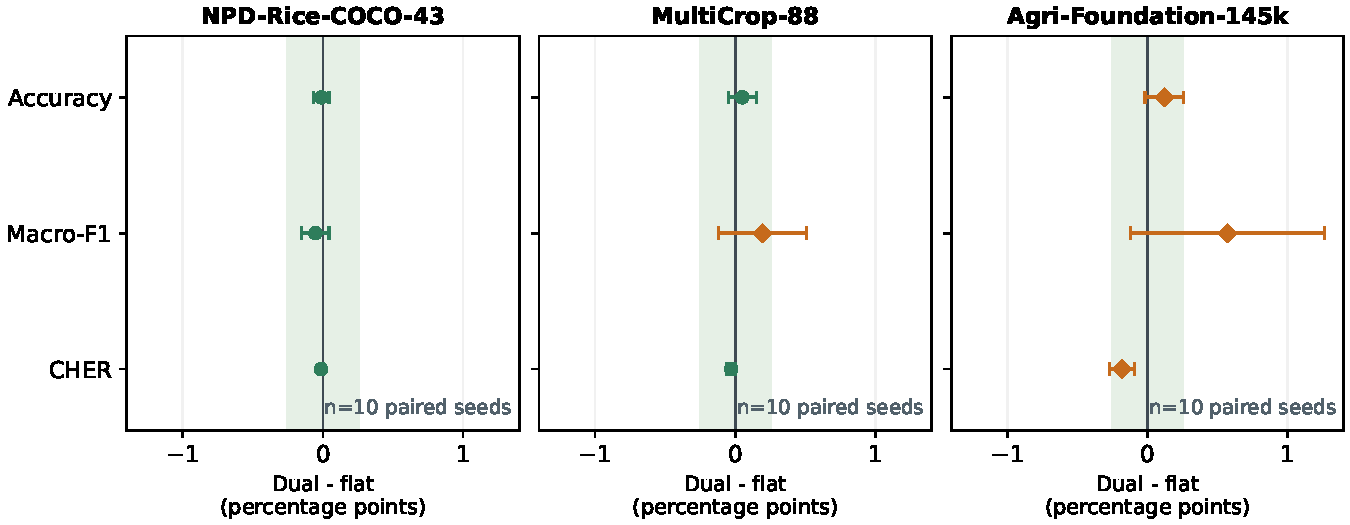
\includegraphics[width=\textwidth]{fig02_core_equivalence_forest.pdf}
\caption{Paired effects for the dual model minus the flat model with 95 percent
confidence intervals. Each dataset has 10 paired seeds. The shaded area marks
the prespecified equivalence region of $\pm0.25$ points. Circles identify
Holm-adjusted equivalence decisions; diamonds identify unresolved decisions. A
negative CHER difference favors the dual model.}
\label{fig:critical-equivalence}
\end{figure*}

The margin analysis showed how the decision changed with the chosen threshold
(Table~\ref{tab:equivalence-sensitivity}). With a $\pm0.10$ point margin,
NPD-Rice-COCO-43 accuracy and CHER and MultiCrop-88 CHER remained equivalent.
With a $\pm0.50$ point margin, accuracy and CHER on Agri-Foundation-145k also
became equivalent. Macro F1 remained unresolved on the two larger taxonomies.
The interpretation of the hardest benchmark therefore depends partly on the
size of an effect judged negligible.

\begin{table*}[htbp]
\centering
\caption{Sensitivity of the Holm-adjusted equivalence decisions to the
absolute margin. Each column applies Holm adjustment across the same nine
dataset and metric decisions. The $\pm0.25$-point column is the predeclared
primary analysis; the other columns are post-hoc sensitivity checks.}
\label{tab:equivalence-sensitivity}
\small
\resizebox{\textwidth}{!}{%
\begin{tabular}{llccc}
\toprule
Dataset & Metric & $\pm0.10$ points & $\pm0.25$ points & $\pm0.50$ points\\
\midrule
NPD-Rice-COCO-43 & Accuracy & Equivalent & Equivalent & Equivalent\\
NPD-Rice-COCO-43 & Macro-F1 & Not established & Equivalent & Equivalent\\
NPD-Rice-COCO-43 & CHER & Equivalent & Equivalent & Equivalent\\
MultiCrop-88 & Accuracy & Not established & Equivalent & Equivalent\\
MultiCrop-88 & Macro-F1 & Not established & Not established & Not established\\
MultiCrop-88 & CHER & Equivalent & Equivalent & Equivalent\\
Agri-Foundation-145k & Accuracy & Not established & Not established & Equivalent\\
Agri-Foundation-145k & Macro-F1 & Not established & Not established & Not established\\
Agri-Foundation-145k & CHER & Not established & Not established & Equivalent\\
\bottomrule
\end{tabular}
}
\end{table*}


CHER counts make the margins easier to interpret. The mean flat and dual counts
were 3.5 and 2.2 errors among 9,333 NPD-Rice-COCO-43 test images, 26.1 and 23.8
among 7,769 MultiCrop-88 images, and 964.5 and 911.4 among 29,041
Agri-Foundation-145k images. A 0.10 point margin equals 9.3, 7.8, and 29.0 events
in these test sets. The primary 0.25 point margin equals 23.3, 19.4, and 72.6
events.

Giving each of the 5,171 NPD-Rice-COCO-43 test families equal total weight did
not alter the comparison. Flat and dual means were 99.033 and 99.020 percent for
accuracy, 98.522 and 98.491 percent for macro F1, and 0.0216 and 0.0107 percent
for CHER. The paired differences were $-0.0129$ points (95 percent CI
$[-0.0829,0.0571]$), $-0.0307$ points ($[-0.1352,0.0739]$), and $-0.0110$
points ($[-0.0241,0.0022]$). Large augmentation families were not responsible
for the near-zero result.

\subsection{Agreement losses}
\label{sec:penalties}

Neither agreement loss improved every dataset and metric
(Table~\ref{tab:critical-clean-penalties}; Fig.~\ref{fig:critical-penalties}).
On NPD-Rice-COCO-43, MAE and KL changed macro F1 by $-0.056$ and $-0.069$ points
compared with the matched dual control. On MultiCrop-88, MAE increased macro F1
by 0.335 points and lowered CHER by 0.021 points. KL changed macro F1 by
$-0.048$ points and lowered CHER by 0.028 points. On Agri-Foundation-145k, KL
produced the largest favorable secondary values: macro F1 rose by 0.419 points
and CHER fell by 0.073 points. The intervals from five seeds were broad,
especially for macro F1, and the directions were not stable across datasets.

\begin{table*}[t]
\centering
\caption{Secondary penalty ablation at consistency weight $\lambda=1$.
All metrics are percentages reported as mean $\pm$ standard deviation over five
matched seeds.}
\label{tab:critical-clean-penalties}
\resizebox{\textwidth}{!}{%
\begin{tabular}{llcccc}
\toprule
Dataset & Configuration & Seeds & Accuracy & Macro-F1 & CHER \\
\midrule
NPD-Rice-COCO-43 & Dual, no penalty & 5 & $99.404 \pm 0.043$ & $98.507 \pm 0.060$ & $0.021 \pm 0.000$ \\
NPD-Rice-COCO-43 & Dual + MAE & 5 & $99.389 \pm 0.039$ & $98.451 \pm 0.116$ & $0.024 \pm 0.005$ \\
NPD-Rice-COCO-43 & Dual + $\mathrm{KL}(q\|p^h)$ & 5 & $99.366 \pm 0.044$ & $98.438 \pm 0.103$ & $0.026 \pm 0.010$ \\
MultiCrop-88 & Dual, no penalty & 5 & $97.657 \pm 0.079$ & $95.156 \pm 0.329$ & $0.304 \pm 0.034$ \\
MultiCrop-88 & Dual + MAE & 5 & $97.732 \pm 0.149$ & $95.491 \pm 0.238$ & $0.283 \pm 0.035$ \\
MultiCrop-88 & Dual + $\mathrm{KL}(q\|p^h)$ & 5 & $97.704 \pm 0.150$ & $95.107 \pm 0.514$ & $0.275 \pm 0.023$ \\
\midrule
Agri-Foundation-145k & Dual, no penalty & 5 & $92.279 \pm 0.092$ & $63.139 \pm 0.548$ & $3.107 \pm 0.056$ \\
Agri-Foundation-145k & Dual + MAE & 5 & $92.124 \pm 0.152$ & $62.689 \pm 0.659$ & $3.208 \pm 0.084$ \\
Agri-Foundation-145k & Dual + $\mathrm{KL}(q\|p^h)$ & 5 & $92.388 \pm 0.036$ & $63.558 \pm 0.205$ & $3.034 \pm 0.052$ \\
\bottomrule
\end{tabular}
}
\end{table*}


\begin{figure*}[htbp]
\centering
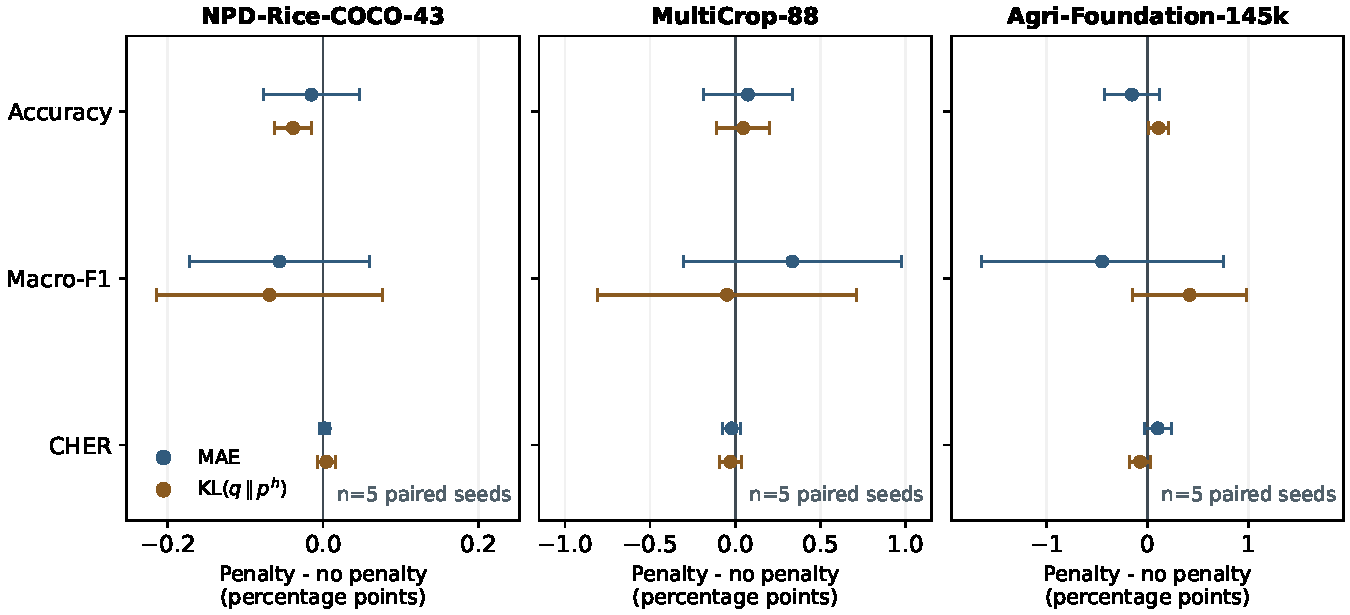
\includegraphics[width=\textwidth]{fig03_clean_penalty_effects.pdf}
\caption{Paired effects of MAE and $\mathrm{KL}(q\|p^h)$ relative to the dual
model without an agreement loss. Points show mean differences and bars show 95
percent confidence intervals from five paired seeds. Positive changes are
favorable for accuracy and macro F1; negative changes are favorable for CHER.}
\label{fig:critical-penalties}
\end{figure*}

\subsection{Head disagreement and predicted-host masking}
\label{sec:tci-hdr-results}

Head disagreement became more frequent as the taxonomy grew
(Table~\ref{tab:tci-hdr}). Mean HDR before TCI was no greater than 0.004 percent
on NPD-Rice-COCO-43, ranged from 0.067 to 0.102 percent on MultiCrop-88, and
ranged from 0.861 to 1.148 percent on Agri-Foundation-145k. TCI reduced HDR to
zero in all 60 dual runs because the condition choice was restricted to the
direct host prediction.

The forced agreement did not yield a stable accuracy gain. Across the nine
combinations of dataset and dual configuration, mean accuracy changes ranged
from $-0.014$ to $+0.018$ points. CHER decreased most on the benchmark with 215
classes: by 0.052 points for KL, 0.100 points for MAE, and 0.137 points for the
dual model without an agreement loss. TCI removed some cross-host errors, but
the small accuracy changes show that a compatible output is not necessarily a
correct output.

\begin{table*}[t]
\centering
\caption{Head disagreement under standard inference and the effect of
taxonomic consistency inference (TCI), implemented as predicted-host masking.
Values are mean $\pm$ standard deviation over
matched runs. Pre-TCI HDR is a percentage; deltas are TCI minus standard
inference in percentage points. The full host-accuracy and macro-F1 results
are provided in Supplementary Table S2.}
\label{tab:tci-hdr}
\small
\resizebox{\textwidth}{!}{%
\begin{tabular}{llrrrr}
\toprule
Dataset & Configuration & Seeds & Pre-TCI HDR & $\Delta$ accuracy & $\Delta$ CHER \\
\midrule
NPD-Rice-COCO-43 & Dual, no penalty & 10 & $0.004 \pm 0.006$ & $0.001 \pm 0.003$ & $-0.001 \pm 0.003$ \\
NPD-Rice-COCO-43 & Dual + MAE & 5 & $0.000 \pm 0.000$ & $0.000 \pm 0.000$ & $0.000 \pm 0.000$ \\
NPD-Rice-COCO-43 & Dual + $\mathrm{KL}(q\|p^h)$ & 5 & $0.002 \pm 0.005$ & $0.002 \pm 0.005$ & $-0.002 \pm 0.005$ \\
\midrule
MultiCrop-88 & Dual, no penalty & 10 & $0.102 \pm 0.026$ & $0.013 \pm 0.033$ & $-0.022 \pm 0.037$ \\
MultiCrop-88 & Dual + MAE & 5 & $0.072 \pm 0.027$ & $-0.005 \pm 0.020$ & $0.008 \pm 0.020$ \\
MultiCrop-88 & Dual + $\mathrm{KL}(q\|p^h)$ & 5 & $0.067 \pm 0.011$ & $0.018 \pm 0.030$ & $-0.021 \pm 0.023$ \\
\midrule
Agri-Foundation-145k & Dual, no penalty & 10 & $1.144 \pm 0.052$ & $0.016 \pm 0.036$ & $-0.137 \pm 0.050$ \\
Agri-Foundation-145k & Dual + MAE & 5 & $1.148 \pm 0.044$ & $-0.002 \pm 0.039$ & $-0.100 \pm 0.044$ \\
Agri-Foundation-145k & Dual + $\mathrm{KL}(q\|p^h)$ & 5 & $0.861 \pm 0.047$ & $-0.014 \pm 0.046$ & $-0.052 \pm 0.031$ \\
\bottomrule
\end{tabular}
}
\end{table*}


For the dual model without a penalty on Agri-Foundation-145k, TCI changed an
average of 332.3 predictions per seed, or 1.144 percent of the test set. Among
these cases, only the direct host head matched the labeled host in 38.7 percent,
only the condition-implied host matched it in 26.8 percent, and both were wrong
in 34.5 percent. TCI gained 79.1 correct top-1 decisions per seed and lost 74.4,
for a net gain of 4.7 cases, or 0.016 points. The small net effect came from
helpful and harmful changes that nearly cancelled each other.

\subsection{Class frequency and labeled-host oracle}
\label{sec:agri-diagnostics}

The class-frequency analysis identified where the numerical dual effect was
concentrated (Table~\ref{tab:agri-diagnostics};
Fig.~\ref{fig:agri-diagnostics}). Mean changes in macro F1 within the four
training-support groups were 0.871 points for 1 to 25 images, 0.600 points for
26 to 100, 0.854 points for 101 to 500, and 0.035 points for more than 500. Only
the 101 to 500 group had a paired 95 percent interval fully above zero
($[0.533,1.176]$). These intervals were exploratory and were not adjusted for
multiple testing. The largest class changes occurred when test support was very
small. \texttt{raspberry\_spot}, for example, gained 23.19 F1 points with four
test images, while \texttt{tomato\_two\_spotted\_spider\_mites} lost 20 points
with one test image. Such values indicate instability and should not be read as
reliable class rankings.

\begin{table*}[htbp]
\centering
\caption{Exploratory diagnostics for Agri-Foundation-145k. Panel A reports
within-bin macro-F1 over 10 paired seeds, where bins are defined by training
images per class. Panel B applies ground-truth-host oracle masking to fixed condition
logits as a non-deployable oracle. Differences are dual minus flat in Panel A
and oracle minus standard in Panel B. Panel A intervals are paired 95\%
confidence intervals across seeds; Panel B reports seed means.}
\label{tab:agri-diagnostics}
\small
\textbf{Panel A: training-frequency strata}\\[2pt]
\resizebox{\textwidth}{!}{%
\begin{tabular}{lrrrrr}
\toprule
Training images/class & Classes & Training images & Flat macro-F1 (\%) & Dual macro-F1 (\%) & Difference (95\% CI), points\\
\midrule
1--25 & 42 & 610 & 30.071 & 30.942 & 0.871 [$-1.677$, 3.419]\\
26--100 & 81 & 4,181 & 52.528 & 53.128 & 0.600 [$-0.174$, 1.374]\\
101--500 & 42 & 7,344 & 75.327 & 76.181 & 0.854 [0.533, 1.176]\\
$>500$ & 50 & 80,436 & 95.745 & 95.780 & 0.035 [$-0.095$, 0.164]\\
\bottomrule
\end{tabular}%
}

\vspace{6pt}
\textbf{Panel B: ground-truth-host oracle}\\[2pt]
\resizebox{\textwidth}{!}{%
\begin{tabular}{lrrrrrr}
\toprule
Configuration & Standard accuracy & Oracle accuracy & $\Delta$ accuracy & Standard macro-F1 & Oracle macro-F1 & $\Delta$ macro-F1\\
\midrule
Flat & 92.151 & 94.445 & 2.294 & 62.645 & 73.246 & 10.601\\
Dual, no penalty & 92.271 & 94.456 & 2.184 & 63.216 & 73.448 & 10.232\\
\bottomrule
\end{tabular}
}
\end{table*}


\begin{figure*}[htbp]
\centering
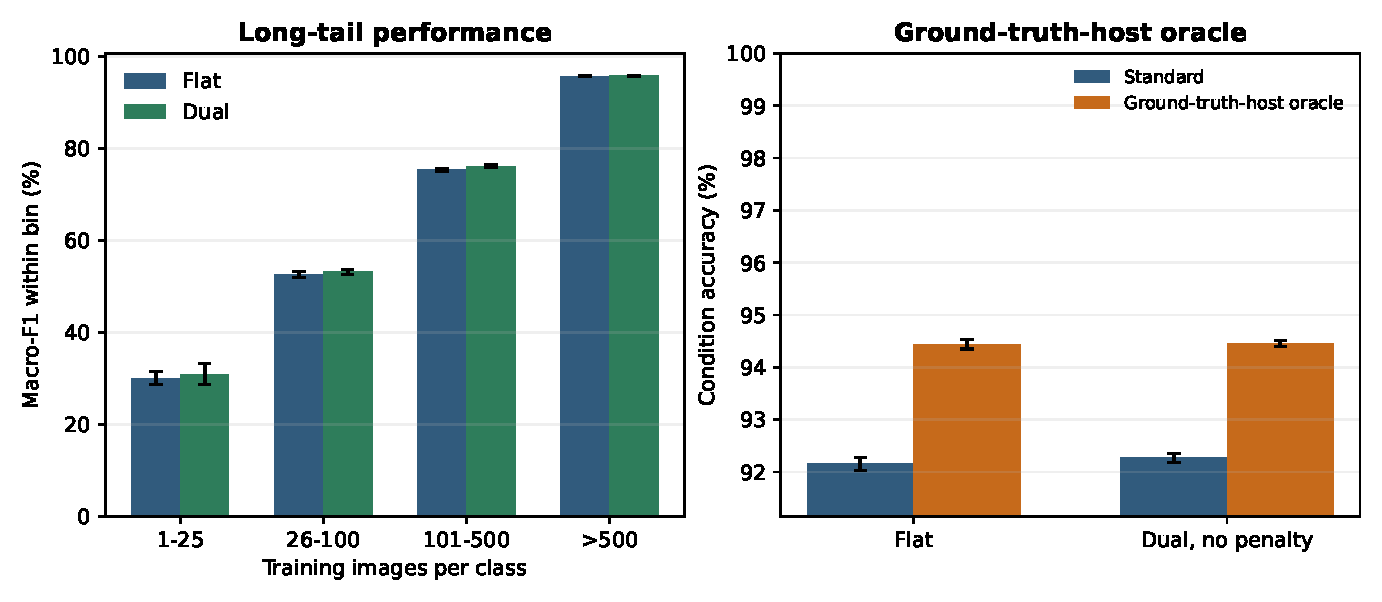
\includegraphics[width=\textwidth]{fig04_agri_long_tail_oracle.pdf}
\caption{Class frequency and labeled-host oracle results for
Agri-Foundation-145k. The left panel shows mean macro F1 within each training
support group over 10 seeds; error bars are 95 percent confidence intervals for
the seed mean. The right panel compares standard condition accuracy with
accuracy after fixed condition logits are restricted by the labeled host. The
oracle is not deployable and sets CHER to zero.}
\label{fig:agri-diagnostics}
\end{figure*}

Several hosts with modest test support accounted for much of the cross-host
error. Flat and dual mean CHER values were 53.5 and 51.4 percent for zucchini
($n=100$), 49.18 and 47.84 percent for bean ($n=134$), 45.65 and 44.26 percent
for plum ($n=115$), and 38.25 and 34.60 percent for tobacco ($n=63$). The
labeled-host oracle raised flat accuracy from 92.151 to 94.445 percent and dual
accuracy from 92.271 to 94.456 percent. Macro F1 rose from 62.645 to 73.246
percent for the flat model and from 63.216 to 73.448 percent for the dual model.
Accurate host information from outside the image classifier could remove a
substantial group of errors. A host predicted from the same image did not
provide the same benefit.

\subsection{Probability quality and selective risk}
\label{sec:calibration-results}

Raw calibration error increased with task difficulty
(Table~\ref{tab:critical-calibration}). ECE was about 0.396 percent on
NPD-Rice-COCO-43, 1.629 to 1.694 percent on MultiCrop-88, and 5.378 to 5.446
percent on Agri-Foundation-145k. Temperature scaling reduced these ranges to
0.192 to 0.220 percent, 0.603 to 0.641 percent, and 1.560 to 1.701 percent. NLL
and Brier score improved for every dataset and configuration.

\begin{table*}[t]
\centering
\caption{Primary-checkpoint probability quality before and after
validation-only temperature scaling. Arrows denote raw $\rightarrow$
temperature-scaled values; entries are means over 10 seeds.}
\label{tab:critical-calibration}
\resizebox{\textwidth}{!}{%
\begin{tabular}{llccccc}
\toprule
Dataset & Configuration & Seeds & ECE (\%) & NLL & Brier & AURC \\
\midrule
NPD-Rice-COCO-43 & Flat & 10 & 0.396$\rightarrow$0.192 & 0.0264$\rightarrow$0.0209 & 0.0100$\rightarrow$0.0096 & 0.0002$\rightarrow$0.0002 \\
NPD-Rice-COCO-43 & Dual, no penalty & 10 & 0.396$\rightarrow$0.220 & 0.0268$\rightarrow$0.0210 & 0.0101$\rightarrow$0.0095 & 0.0002$\rightarrow$0.0002 \\
MultiCrop-88 & Flat & 10 & 1.694$\rightarrow$0.641 & 0.1314$\rightarrow$0.0883 & 0.0403$\rightarrow$0.0371 & 0.0014$\rightarrow$0.0016 \\
MultiCrop-88 & Dual, no penalty & 10 & 1.629$\rightarrow$0.603 & 0.1275$\rightarrow$0.0854 & 0.0388$\rightarrow$0.0360 & 0.0013$\rightarrow$0.0014 \\
Agri-Foundation-145k & Flat & 10 & 5.446$\rightarrow$1.701 & 0.4749$\rightarrow$0.3114 & 0.1300$\rightarrow$0.1139 & 0.0072$\rightarrow$0.0073 \\
Agri-Foundation-145k & Dual, no penalty & 10 & 5.378$\rightarrow$1.560 & 0.4569$\rightarrow$0.2971 & 0.1278$\rightarrow$0.1114 & 0.0071$\rightarrow$0.0071 \\
\bottomrule
\end{tabular}
}
\end{table*}


\begin{figure*}[htbp]
\centering
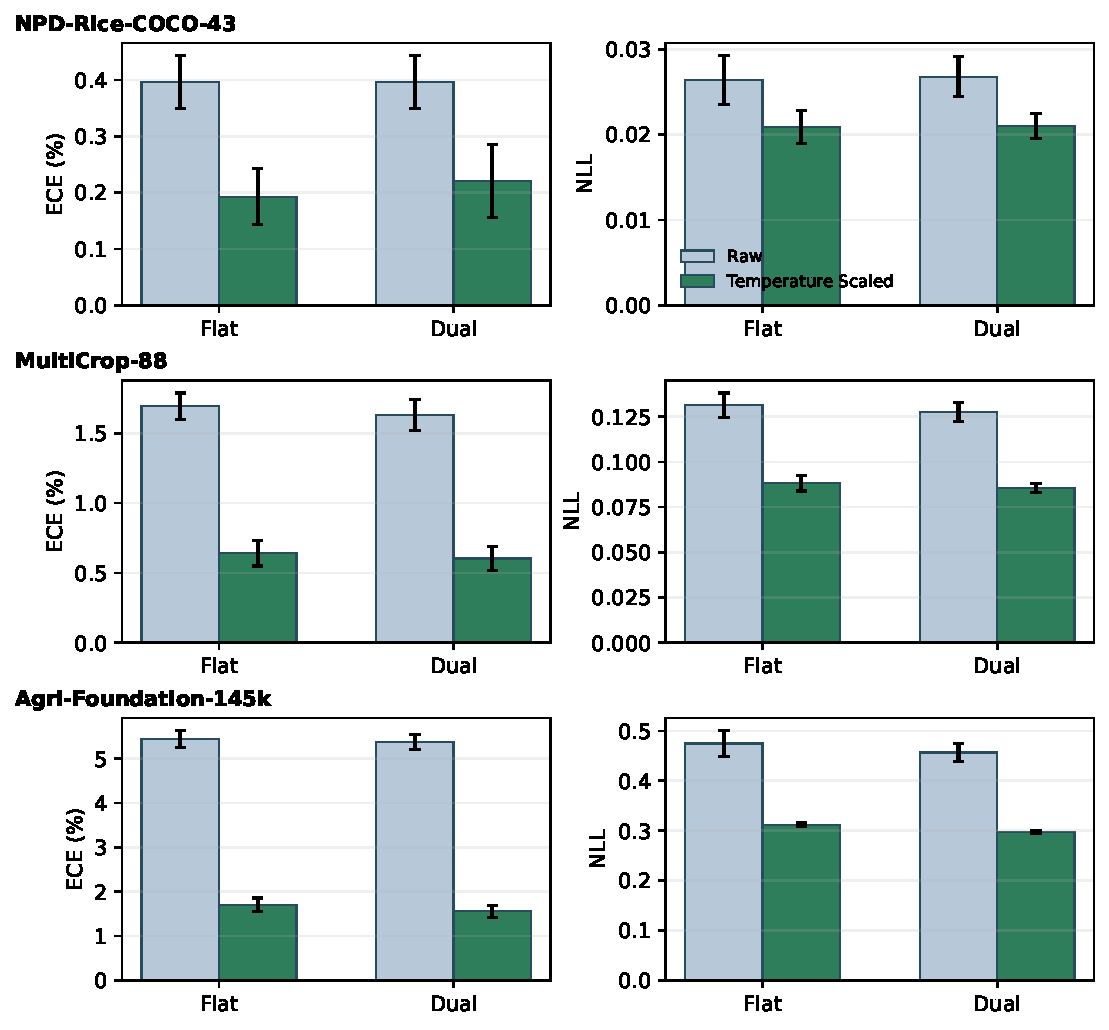
\includegraphics[width=\textwidth]{fig05_controlled_probability_quality.pdf}
\caption{Expected calibration error and negative log likelihood before and
after temperature scaling fitted on validation data. Bars show means over 10
seeds; error bars show standard deviations across seeds.}
\label{fig:probability-quality}
\end{figure*}

AURC changed little because a single temperature does not materially reorder
confidence scores. The flat and dual risk-coverage curves were also close
within each dataset (Fig.~\ref{fig:risk-coverage}). Referral based on confidence
could reduce error among retained cases in this retrospective analysis. The
curves do not include reviewer capacity, review cost, or the accuracy of the
person who receives a referred image.

\begin{figure*}[htbp]
\centering
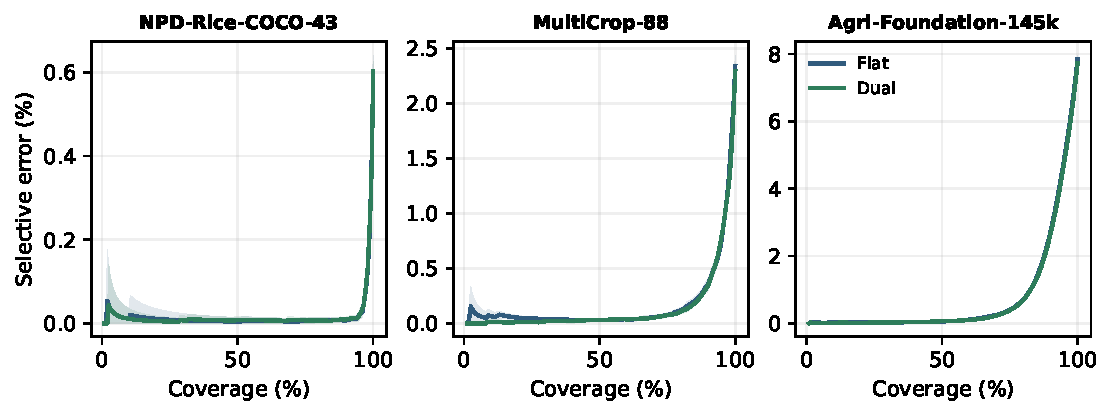
\includegraphics[width=\textwidth]{fig06_controlled_risk_coverage.pdf}
\caption{Selective condition error after temperature scaling as retained
coverage changes. Lines show seed means for the primary flat and dual models;
shaded bands show 95 percent confidence intervals across seeds. Lower error is
better.}
\label{fig:risk-coverage}
\end{figure*}

\section{Discussion}
\label{sec:discussion}

\subsection{What the host head changed}

The host head produced no stable improvement in condition recognition.
NPD-Rice-COCO-43 showed practical equivalence for all three primary outcomes.
MultiCrop-88 showed equivalence for accuracy and CHER, while macro F1 remained
unresolved. The largest numerical changes appeared on Agri-Foundation-145k,
but the uncertainty was too wide to support either equivalence at the primary
margin or a broad claim that the dual model was better. The gap of nearly 29
points between accuracy and macro F1 on this dataset also confirms that overall
accuracy alone is inadequate for a large imbalanced taxonomy.

The frequency and oracle analyses explain why host information can still
matter. The clearest descriptive increase for the dual model occurred among
classes with 101 to 500 training images. Results for the rarest classes varied
widely because some test classes contained only one to four images. When the
true host was supplied as an oracle, both models gained about 2.2 accuracy
points and more than 10 macro F1 points. Reliable crop metadata can thus be
useful. That benefit cannot be attributed to a host head trained from the same
joint label and the same image features.

\subsection{Agreement and correctness are different questions}

HDR records conflicts before a rule is applied. TCI removes those conflicts by
forcing the condition decision into the host selected by the direct head. An
HDR after TCI of zero is guaranteed, so it says nothing by itself about whether
the condition is correct. On Agri-Foundation-145k, TCI changed hundreds of
predictions per seed, yet the gains and losses almost balanced. Reporting only
the final agreement would hide this exchange. A useful audit should include HDR
before masking together with the changes in accuracy, macro F1, and CHER.

The MAE and KL results lead to the same interpretation. Both losses encourage
two probability distributions to agree, but both distributions ultimately come
from targets contained in the same joint label. Once condition and host cross
entropy have largely aligned the heads, another agreement term can change the
optimization path without adding new information. The mixed effects from five
seeds, along with different gradient scales under a common unit coefficient, do
not support either loss as a generally useful addition.

\subsection{Identity controls and uncertainty}

The data checks define the scope of the comparison. Related augmented files
were kept together in NPD-Rice-COCO-43. MultiCrop-88 was cleaned for exact
duplicates and conflicting hashes. The Agri-Foundation-145k test set had no
exact match in the development pool. Family weighting also showed that large
augmentation groups did not drive the NPD-Rice-COCO-43 result. Fixed manifests
and paired seeds make each model comparison traceable.

These checks cannot rule out every visually related image. MultiCrop-88 lacks
independent acquisition provenance, and exact hashing cannot find a resized,
cropped, or recompressed copy. The synthetic development placeholder in
Agri-Foundation-145k creates a separate problem because one class has no real
development image. Since the same derivative was used for all configurations,
the paired architecture comparison is still matched. Absolute macro F1 and the
result for that class should not be generalized. The supplied class-exclusion
script needs to be run and its output deposited before submission.

Equivalence testing also changed how the numerical differences should be read.
A large $p$ value would only show that a difference was not detected. The
prespecified margin allowed a direct test of whether the whole plausible effect
was small enough to ignore. The two sensitivity margins show which decisions
remain stable and which depend on accepting a larger effect as negligible.

\subsection{Confidence and use in practice}

Temperature scaling was the only adjustment that improved all primary settings
for ECE, NLL, and Brier score. This matters when probabilities are displayed to
users or used for referral. The nearly unchanged AURC provides a useful limit:
calibration made the probability values more faithful, but it did not make the
model better at ranking easy and difficult images. It also did not correct
wrong labels or demonstrate safety in field use.

These findings suggest a practical evaluation sequence. A host-aware model
should first be compared with a flat baseline using the same seeds and a margin
chosen before test results are examined. If the host head is retained for
audit, disagreement should be reported before a taxonomy rule is applied. Any
masking step should then be assessed by the correct decisions it gains and
loses. A predicted host should not be described as independent crop evidence.
When confidence will control acceptance or referral, calibration should be
fitted on validation data and tested on untouched outputs.

Although the experiments used Swin Small, the same logic applies to other
models whenever one level of a label hierarchy is determined by another. In
such a setting, split identity, paired uncertainty, direct equivalence tests,
unmasked head disagreement, and calibrated probabilities provide more
information than a single best run.

\section{Scope and limitations}
\label{sec:limitations}

This work evaluates performance within three fixed datasets. It does not test
transfer across data sources, seasons, geographic regions, devices, or field
conditions. The three datasets are local derivatives with different class
counts, host counts, imbalance, provenance, and visual properties.
NPD-Rice-COCO-43 has source-family controls. MultiCrop-88 and
Agri-Foundation-145k have exact-byte checks but no perceptual hash or embedding
similarity analysis. The supervised COCO background class was represented
during training and must not be described as open-set recognition or as general
detection of inputs outside the training distribution.

The Agri-Foundation-145k derivative contains a synthetic $10\times10$
development placeholder as the only development support for one class. This
limits the interpretation of absolute macro F1 and class-specific performance.
No class-exclusion result is reported because the output from the available
sensitivity script was absent from the supplied archive. That analysis should
be run, checked, and included in the permanent repository. The present
comparisons remain matched because all models were trained and tested on the
same locked cases.

The intervals from 10 seeds quantify variation from fine-tuning on fixed test
sets; they do not quantify uncertainty over new populations. Macro F1 intervals
on the benchmark with 215 classes are broad. The host loss weight was fixed at
$\alpha=1$, and the MAE and KL analyses used five seeds with $\lambda=1$.
Other weights may behave differently. TCI uses a host predicted from the same
representation, while the labeled-host oracle is not deployable. Analyses by
frequency, class, host, and disagreement type were exploratory, and some of the
largest class effects came from very small test supports.

Swin Small was pretrained on natural images. The findings concern fine-tuning
this backbone and do not cover training from scratch or every possible
architecture. Calibration and selective risk were evaluated retrospectively.
No field workflow, specialist review process, latency constraint, user study,
or agronomic outcome was tested.

\section{Conclusion}
\label{sec:conclusion}

Across 90 controlled runs, crop host supervision with equal loss weight did not
provide a dependable advantage over a flat Swin Small classifier. All primary
outcomes were equivalent on NPD-Rice-COCO-43. Accuracy and CHER were equivalent
on MultiCrop-88, while the remaining outcomes were unresolved at the
$\pm0.25$ point margin. Neither agreement loss improved every dataset and
metric. Predicted-host masking removed head conflicts but had little effect on
accuracy. In contrast, the labeled-host oracle improved accuracy on the
benchmark with 215 classes by about 2.2 points. Independent host information can
be useful, but agreement produced from the model's own host prediction is not
an independent check of correctness. Temperature scaling gave the most
consistent improvement in probability quality. Under the tested conditions,
the host head is better viewed as an audit channel than as a reliable route to
higher condition accuracy.

\section*{Data and code availability}

Code for training, evaluation, statistical analysis, and figure generation is
maintained in a private GitHub repository:
\url{https://github.com/omair-khan2232/Auditing-crop-host-supervision}.
Reviewer access will be provided on special permission through the authors or
the editorial office during peer review. The repository contains the exact
split manifests, ordered taxonomies, configuration records, metrics for each
seed, figure scripts, artifact hashes, and the Agri-Foundation-145k
placeholder-class sensitivity output described in the Supplementary Material.
The image datasets are not redistributed because each source has its own
license and terms. Logits and checkpoints should be deposited separately where
the source terms and storage limits allow.

\section*{CRediT authorship contribution statement}

Muhammad Omair Khan and Muhammad Ahmad contributed equally to this work.
Muhammad Omair Khan: Conceptualization, Methodology, Software, Validation,
Formal analysis, Investigation, Data curation, Visualization, Writing - original
draft. Muhammad Ahmad: Conceptualization, Methodology, Software, Validation,
Formal analysis, Investigation, Data curation, Visualization, Writing - original
draft. MD Ariful Islam Mozumder: Methodology, Validation, Resources, Writing -
review and editing. Hee-Cheol Kim: Supervision, Project administration,
Resources, Writing - review and editing, Corresponding author.

\section*{Funding}

This work was supported by the Institute of Information \& Communications
Technology Planning \& Evaluation (IITP)--Innovative Human Resource Development
for Local Intellectualization program grant funded by the Korea government
(MSIT) (IITP-2024-RS-2024-00436773).

\section*{Declaration of competing interest}

The authors declare that they have no known competing financial interests or
personal relationships that could have appeared to influence the work reported
in this paper.

\section*{Acknowledgments}

The authors gratefully acknowledge the support provided by IITP and MSIT
through the Innovative Human Resource Development for Local Intellectualization
program.

\section*{Declaration of generative AI and AI-assisted technologies in the
manuscript preparation process}

% Before submission, verify whether the journal requires the exact LLM service, provider, version, and date in this declaration.
During preparation of this work, the authors used a large language model (LLM)
for language editing, manuscript organization, reference checking, LaTeX
preparation, code review, and figure preparation. The authors reviewed and
edited the resulting material, checked the references and numerical statements
against the source files and stored results, and take full responsibility for
the content of the article.

\bibliographystyle{elsarticle-num}
\begin{thebibliography}{31}

\bibitem{hughes2015}
D.~P. Hughes, M.~Salath\'e, An open access repository of images on plant health
to enable the development of mobile disease diagnostics, arXiv:1511.08060
(2015). \url{https://doi.org/10.48550/arXiv.1511.08060}.

\bibitem{mohanty2016}
S.~P. Mohanty, D.~P. Hughes, M.~Salath\'e, Using deep learning for image-based
plant disease detection, Frontiers in Plant Science 7 (2016) 1419.
\url{https://doi.org/10.3389/fpls.2016.01419}.

\bibitem{ferentinos2018}
K.~P. Ferentinos, Deep learning models for plant disease detection and
diagnosis, Computers and Electronics in Agriculture 145 (2018) 311--318.
\url{https://doi.org/10.1016/j.compag.2018.01.009}.

\bibitem{barbedo2018}
J.~G.~A. Barbedo, Impact of dataset size and variety on the effectiveness of
deep learning and transfer learning for plant disease classification,
Computers and Electronics in Agriculture 153 (2018) 46--53.
\url{https://doi.org/10.1016/j.compag.2018.08.013}.

\bibitem{gui2021}
P.~Gui, W.~Dang, F.~Zhu, Q.~Zhao, Towards automatic field plant disease
recognition, Computers and Electronics in Agriculture 191 (2021) 106523.
\url{https://doi.org/10.1016/j.compag.2021.106523}.

\bibitem{dosovitskiy2021}
A.~Dosovitskiy et al., An image is worth 16$\times$16 words: Transformers for
image recognition at scale, in: International Conference on Learning
Representations, 2021.

\bibitem{liu2021swin}
Z.~Liu et al., Swin Transformer: Hierarchical vision transformer using shifted
windows, in: Proceedings of the IEEE/CVF International Conference on Computer
Vision, 2021, pp. 10012--10022.
\url{https://doi.org/10.1109/ICCV48922.2021.00986}.

\bibitem{fu2024}
L.~Fu et al., Crop pest image recognition based on the improved ViT method,
Information Processing in Agriculture 11 (2) (2024) 249--259.
\url{https://doi.org/10.1016/j.inpa.2023.02.007}.

\bibitem{ngugi2021}
L.~C. Ngugi, M.~Abelwahab, M.~Abo-Zahhad, Recent advances in image processing
techniques for automated leaf pest and disease recognition: A review,
Information Processing in Agriculture 8 (1) (2021) 27--51.
\url{https://doi.org/10.1016/j.inpa.2020.04.004}.

\bibitem{elhanafy2026}
A.~El Hanafy, A.~Hessane, Y.~Farhaoui, Exploring attention mechanisms in deep
learning for plant health: A scoping review on disease and pest detection,
Information Processing in Agriculture (2026), in press.
\url{https://doi.org/10.1016/j.inpa.2026.05.006}.

\bibitem{caruana1997}
R.~Caruana, Multitask learning, Machine Learning 28 (1997) 41--75.
\url{https://doi.org/10.1023/A:1007379606734}.

\bibitem{silla2011}
C.~N. Silla Jr., A.~A. Freitas, A survey of hierarchical classification across
different application domains, Data Mining and Knowledge Discovery 22 (2011)
31--72. \url{https://doi.org/10.1007/s10618-010-0175-9}.

\bibitem{picon2019}
A.~Picon, M.~Seitz, A.~Alvarez-Gila, P.~Mohnke, A.~Ortiz-Barredo,
J.~Echazarra, Crop conditional convolutional neural networks for massive
multi-crop plant disease classification over cell phone acquired images taken
on real field conditions, Computers and Electronics in Agriculture 167 (2019)
105093. \url{https://doi.org/10.1016/j.compag.2019.105093}.

\bibitem{yao2024}
J.~Yao, S.~N. Tran, S.~Garg, S.~Sawyer, Deep learning for plant identification
and disease classification from leaf images: Multi-prediction approaches, ACM
Computing Surveys 56 (6) (2024) Article 153.
\url{https://doi.org/10.1145/3639816}.

\bibitem{ergun2026}
E.~Erg\"un, H.~Okumu\c{s}, Robust eggplant disease recognition using a
learnable weighted deep ensemble with test-time augmentation, Information
Processing in Agriculture (2026), in press.
\url{https://doi.org/10.1016/j.inpa.2026.03.010}.

\bibitem{singh2026}
C.~Singh, A.~Singh, S.~Dhelim, Neuro-symbolic AI for rice disease diagnosis
with calibrated attention and rule-aware explanations, Information Processing
in Agriculture (2026), in press.
\url{https://doi.org/10.1016/j.inpa.2026.02.006}.

\bibitem{kapoor2023}
S.~Kapoor, A.~Narayanan, Leakage and the reproducibility crisis in
machine-learning-based science, Patterns 4 (9) (2023) 100804.
\url{https://doi.org/10.1016/j.patter.2023.100804}.

\bibitem{bouthillier2021}
X.~Bouthillier et al., Accounting for variance in machine learning benchmarks,
Proceedings of Machine Learning and Systems 3 (2021).
\url{https://proceedings.mlsys.org/paper_files/paper/2021/hash/0184b0cd3cfb185989f858a1d9f5c1eb-Abstract.html}.

\bibitem{loshchilov2019}
I.~Loshchilov, F.~Hutter, Decoupled weight decay regularization, in:
International Conference on Learning Representations, 2019.

\bibitem{guo2017}
C.~Guo, G.~Pleiss, Y.~Sun, K.~Q. Weinberger, On calibration of modern neural
networks, in: Proceedings of the 34th International Conference on Machine
Learning, 2017, pp. 1321--1330.
\url{https://proceedings.mlr.press/v70/guo17a.html}.

\bibitem{brier1950}
G.~W. Brier, Verification of forecasts expressed in terms of probability,
Monthly Weather Review 78 (1) (1950) 1--3.
\url{https://doi.org/10.1175/1520-0493(1950)078<0001:VOFEIT>2.0.CO;2}.

\bibitem{geifman2017}
Y.~Geifman, R.~El-Yaniv, Selective classification for deep neural networks,
in: Advances in Neural Information Processing Systems 30, 2017,
pp. 4885--4894.

\bibitem{lakens2017}
D.~Lakens, Equivalence tests: A practical primer for $t$ tests, correlations,
and meta-analyses, Social Psychological and Personality Science 8 (4) (2017)
355--362. \url{https://doi.org/10.1177/1948550617697177}.

\bibitem{holm1979}
S.~Holm, A simple sequentially rejective multiple test procedure,
Scandinavian Journal of Statistics 6 (2) (1979) 65--70.

\bibitem{newplantdiseases}
[dataset] S.~Bhattarai, New Plant Diseases Dataset, Kaggle dataset.
\url{https://www.kaggle.com/datasets/vipoooool/new-plant-diseases-dataset}
(accessed 21 August 2026).

\bibitem{riceleafs}
[dataset] S.~Riyaz, Rice Leafs: An image collection of four rice leaf
conditions, Kaggle dataset, 2019.
\url{https://www.kaggle.com/datasets/shayanriyaz/riceleafs}
(accessed 21 August 2026).

\bibitem{lin2014}
T.-Y. Lin et al., Microsoft COCO: Common objects in context, in: European
Conference on Computer Vision, 2014, pp. 740--755.
\url{https://doi.org/10.1007/978-3-319-10602-1_48}.

\bibitem{coco2014kaggle}
[dataset] Kaggle user jeffaudi, COCO 2014 Dataset (for YOLOv3), Kaggle dataset.
\url{https://www.kaggle.com/datasets/jeffaudi/coco-2014-dataset-for-yolov3}
(accessed 24 August 2026).

\bibitem{ahamed2024}
M.~F. Ahamed, A.~Salam, M.~Nahiduzzaman, M.~Abdullah-Al-Wadud,
S.~M.~R. Islam, Streamlining plant disease diagnosis with convolutional neural
networks and edge devices, Neural Computing and Applications 36 (2024)
18445--18477. \url{https://doi.org/10.1007/s00521-024-10152-y}.

\bibitem{dobrovsky_multicrop}
[dataset] A.~Dobrovsky, Plant Disease Classification Merged Dataset,
Kaggle dataset.
\url{https://www.kaggle.com/datasets/alinedobrovsky/plant-disease-classification-merged-dataset}
(accessed 24 August 2026).

\bibitem{agrifoundation_hf}
[dataset] M.~Bekhouche, S.~Zertal, Agri-Foundation-v1,
Hugging Face dataset.
\url{https://huggingface.co/datasets/mbsoft31/agri-foundation-v1}
(accessed 24 August 2026).

\bibitem{agrifoundation2026}
[dataset] M.~Bekhouche, S.~Zertal, Agri-Foundation-145k: A unified large-scale
dataset for agricultural disease detection, Zenodo, version 1 (2026).
\url{https://doi.org/10.5281/zenodo.18214758}.

\bibitem{russakovsky2015}
O.~Russakovsky et al., ImageNet large scale visual recognition challenge,
International Journal of Computer Vision 115 (2015) 211--252.
\url{https://doi.org/10.1007/s11263-015-0816-y}.

\end{thebibliography}
\end{document}
